\documentclass{article}
\usepackage{graphicx} % Required for inserting images

\usepackage[a4paper,
            bindingoffset=0.2in,
            left=1in,
            right=1in,
            top=1in,
            bottom=1in,
            footskip=.25in]{geometry}

\usepackage{amsmath}
\usepackage{amssymb}
\usepackage{amsfonts}
\title{TP AMS307}
\author{Thibault Mougin}
\date{February 2024}

\begin{document}

\maketitle

\section{Introduction}
On introduit la géométrie suivante : 
\begin{figure}[htbp]
    \centering
    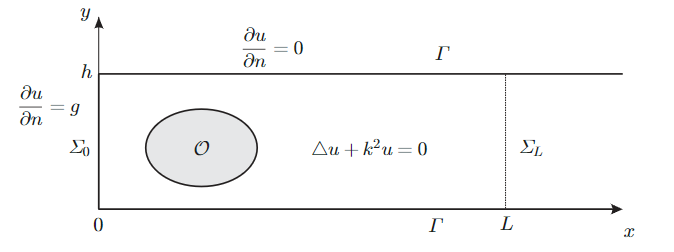
\includegraphics[trim ={0 0.2cm 0 0cm},clip, scale=0.5]{image(1).png}
\end{figure}

où l'on cherche à résoudre ce problème : \\

\begin{tabular}{|ll|}
\hline 
& \\
$ \displaystyle \Delta u+k^2 u=0$ & sur $\Omega$ \\
& \\
$\displaystyle \frac{\partial u}{\partial n}=0$ & sur $\Gamma \cup \partial \mathcal{O}$ \\
& \\
$\displaystyle \frac{\partial u}{\partial n}=g$ & sur $\Sigma_0$ \\
& \\
$\displaystyle u(x, y)=\sum_{n \geq 0} \alpha_n e^{i \beta_n x} \varphi_n(y)$ & $\forall x>L \quad$ (condition de rayonnement)\\
& \\
\hline 
\end{tabular} \vskip 0.2in 
où $\displaystyle \beta_n=\sqrt{k^2-\left(\frac{n \pi}{h}\right)^2}$ avec $\mathcal{I} m \beta_n \geq 0$ et $\mathcal{R} e \beta_n \geq 0$
 \\ \null \quad \; $\displaystyle \varphi_n(y)=a_n \cos \left(\frac{n \pi y}{h}\right)$ avec $\displaystyle a_n=\sqrt{\frac{2}{h}}$ si $n>0$ et $\displaystyle a_0=\sqrt{\frac{1}{h}}$. \\
 

\section{Réduction à un domaine borné}
\subsection{Approximation basse fréquence}
\subsubsection{Formulation variationnelle}
Lorsque $ k < \frac{\pi}{h}$, on introduit le problème approché suivant dans $\left.\Omega_a=\Omega \cap\right] 0, a[\times] 0, h[$ :
$$
\begin{cases}\displaystyle \Delta u+k^2 u=0 & \text { sur } \Omega_a \\[0.2cm] \displaystyle  \frac{\partial u}{\partial n}=0 & \text { sur } \Gamma \cup \partial \mathcal{O} \\[0.4cm] \displaystyle \frac{\partial u}{\partial n}=g & \text { sur } \Sigma_0 \\[0.4cm] \displaystyle  \frac{\partial u}{\partial n}=i k u & \text { sur } \Sigma_a(a>L) .\end{cases}
$$
La formulation variationnelle associée est donnée par: \bigbreak
Trouver $p \in H^1\left(\Omega_a\right)$, tel que $\forall q \in H^1\left(\Omega_a\right)$,
$$
\int_{\Omega_a}\left(\nabla p \cdot \nabla \bar{q}-k^2 p \bar{q}\right)-\mathrm{i} k \int_{\Sigma_a} p \bar{q}=\int_{\Sigma_{0}} g \bar{q} .
$$ 
\subsubsection{Résultats numériques}

On trace sur la figure 1 les parties réelles et imaginaires de $u$, solution du problème approché basse fréquence pour $ k = 3 < \frac{\pi}{h}$ : les conditions aux limites semblent respectées, l'allure dans loin de la perturbation a l'air correcte. \\
Sur la figure 2, on trace la différence entre la solution $u$ obtenue par approximation basse fréquence et celle que l'on obtient avec l'opérateur DtN tronqué à 10 modes, notée $u_{10}$ (on place $\Sigma_a$ \textit{assez loin} de la perturbation et $N=10$ nous fournit alors une solution \textit{quasi-exacte}). On observe que l'approximation basse fréquence fournit une solution acceptable : l'influence des modes d'ordre élevés ne se voit vraiment qu'au voisinage de $\Sigma_a$ et l'erreur est de l'ordre de $10^{-4}$ partout ailleurs.

\begin{figure}[h!]
    \centering
    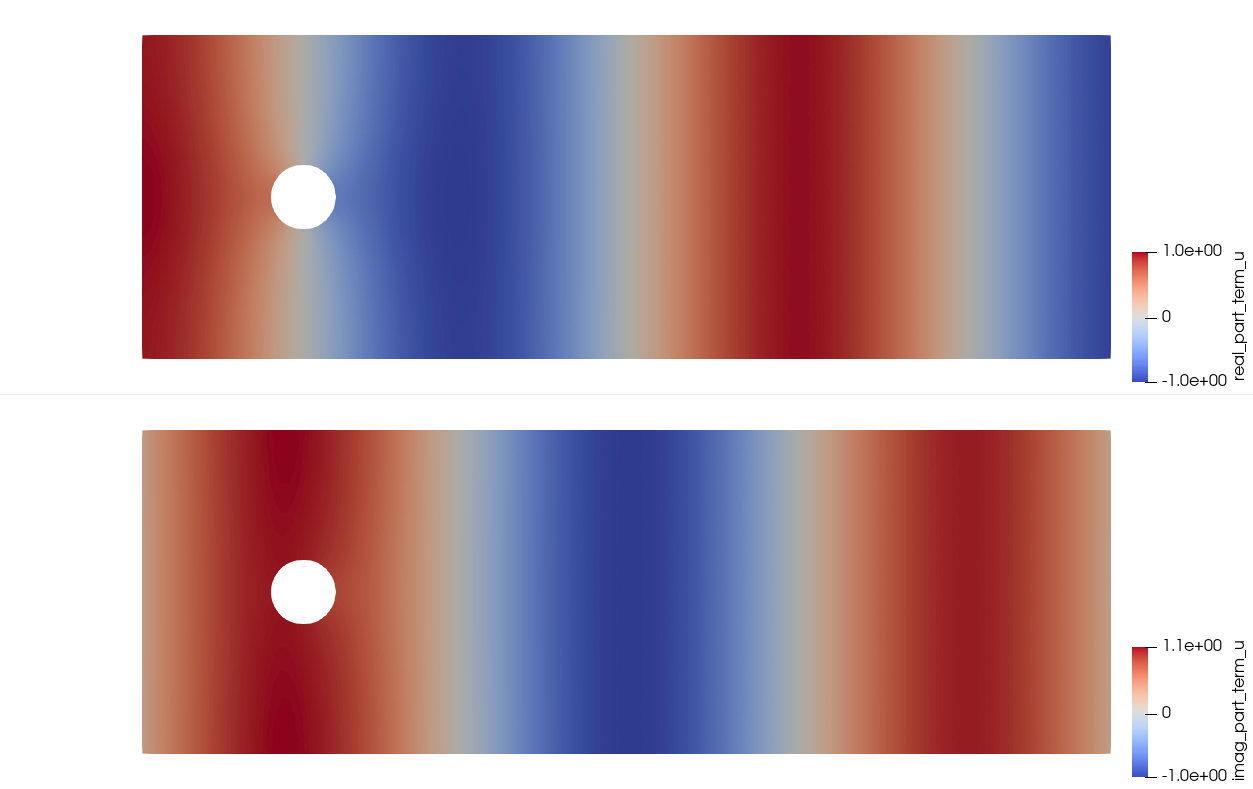
\includegraphics[scale=0.3]{sc_LF_k3_b3.png}
    \caption{$\mathfrak{Re }\; u$ (haut), $\mathfrak{Im }\; u$ (bas), approximation basse fréquence, $k=3$, $h=1$,  $a=3$}
\end{figure}

\begin{figure}[h!]
    \centering
    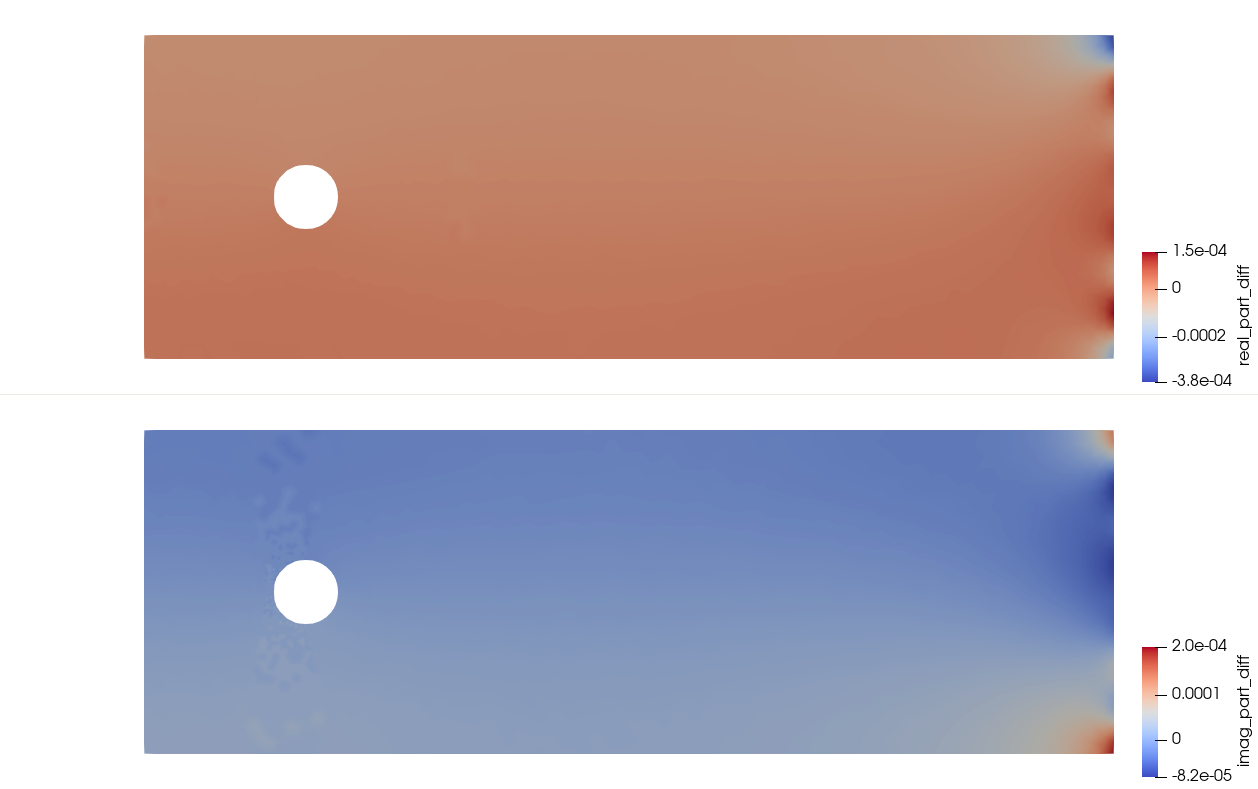
\includegraphics[scale=0.3]{sc_diff_LF_DtN10_k3_b3.png}
    \caption{$\mathfrak{Re }\; (u-u_{10})$ (haut), $\mathfrak{Im }\; (u-u_{10})$ (bas), $k=3$, $h=1$,  $a=3$}
\end{figure}

\newpage
\subsection{Méthode DtN}
\subsubsection{Formulation variationnelle}



On introduit l'opérateur DtN tronqué au rang $N$ usuel : $$T_n u=\sum_{0 \leq n \leq N} i \beta_n\left(\int_{\Sigma_a} u \varphi_n\right) \varphi_n(y) \text { sur } \Sigma_a \quad (a>L) $$

Le problème approché est alors :
$$
\begin{cases} \displaystyle \Delta u+k^2 u=0 & \text { sur } \Omega_a \\[0.2cm] \displaystyle  \frac{\partial u}{\partial n}=0 & \text { sur } \Gamma \cup \partial \mathcal{O} \\[0.4cm] \displaystyle  \frac{\partial u}{\partial n}=g & \text { sur } \Sigma_0 \\[0.4cm] \displaystyle  \frac{\partial u}{\partial n}=T_Nu & \text { sur } \Sigma_a(a>L) .\end{cases}
$$
La formulation variationnelle associée est donnée par: \bigbreak
Trouver $p \in H^1\left(\Omega_a\right)$, tel que $\forall q \in H^1\left(\Omega_a\right)$,
$$
\int_{\Omega_a}\left(\nabla p \cdot \nabla \bar{q}-k^2 p \bar{q}\right)-\int_{\Sigma_a}T_N p\bar{q}=\int_{\Sigma_{0}} g \bar{q} .
$$ 

\subsubsection{Résultats numériques}

On trace sur la figure 3 les parties réelles et imaginaires de $u_4$, solution du problème avec DtN, avec $k=10$, $N=4$ et $a=2$. \\
Sur la figure 4, on trace la différence entre la solution $u_4$ obtenue pour $N=4$ et $u_{16}$ avec $N=16$. On observe qu'augmenter $N$ au delà de $4$ n'a pas d'effet sur la résolution au voisinage de la perturbation..


\begin{figure}[h!]
\begin{minipage}[b]{.4\textwidth}
\centering
    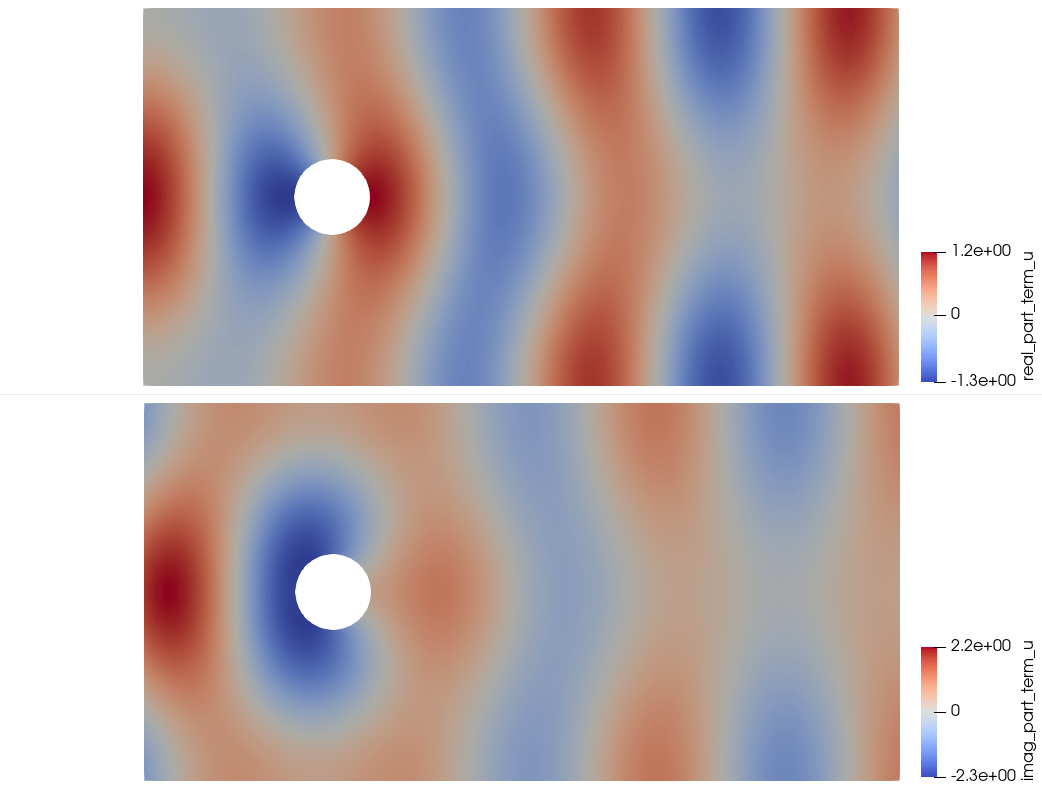
\includegraphics[trim = {5cm 0cm 0cm 0cm}, clip, scale=0.25]{sc_DtN_2_4.png}
    \caption{$\mathfrak{Re }\; u_4$ (haut), $\mathfrak{Im }\; u_4$ (bas), $k=10$, $h=1$,  $a=2$}
\end{minipage}
\hfill
\begin{minipage}[b]{.45\textwidth}
 \centering
    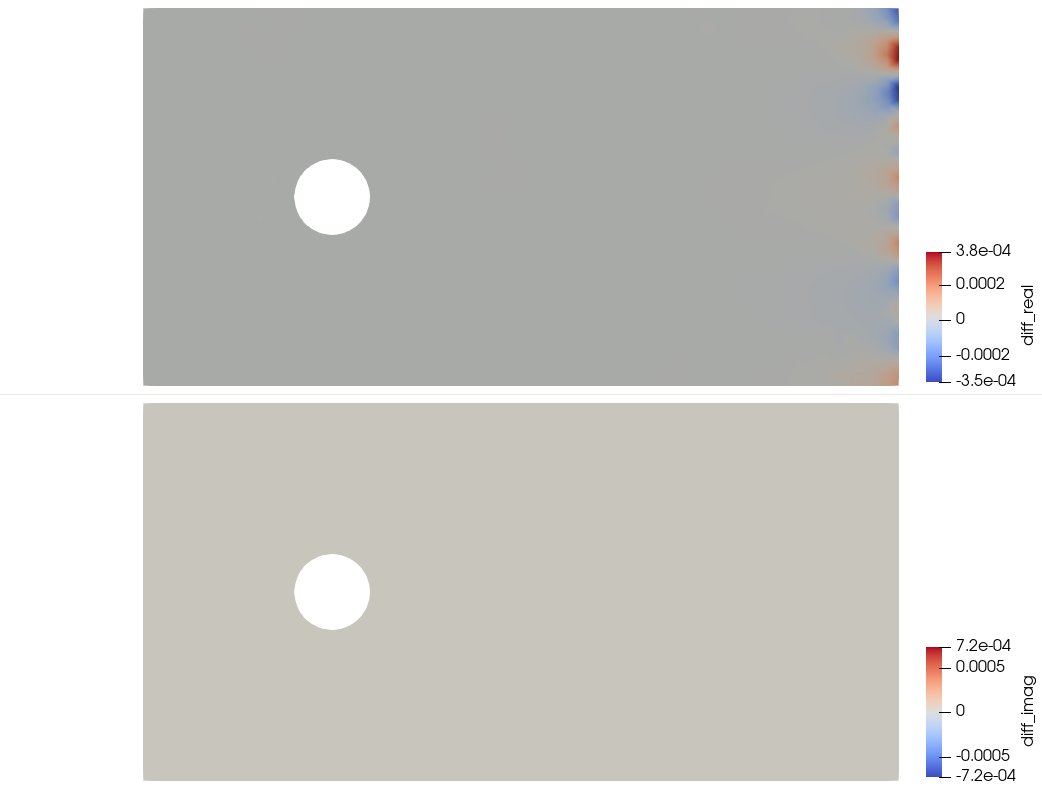
\includegraphics[trim = {5cm 0cm 0cm 0cm}, clip, scale=0.25]{sc_DtN_2_diff_4_16.png}
    \caption{$\mathfrak{Re }\; (u_{4}-u_{16})$ (haut), $\mathfrak{Im }\; (u_{4}-u_{16})$ (bas), $k=10$, $h=1$,  $a=2$}
\end{minipage}
\end{figure}
\newpage
Pour $a=1$, en revanche, on aurait intérêt à augmenter $N$ : on voit ici que $N=4$ n'est pas suffisant pour éliminer les reflexions parasites vers la perturbation : 

\begin{figure}[h!]
    \centering
    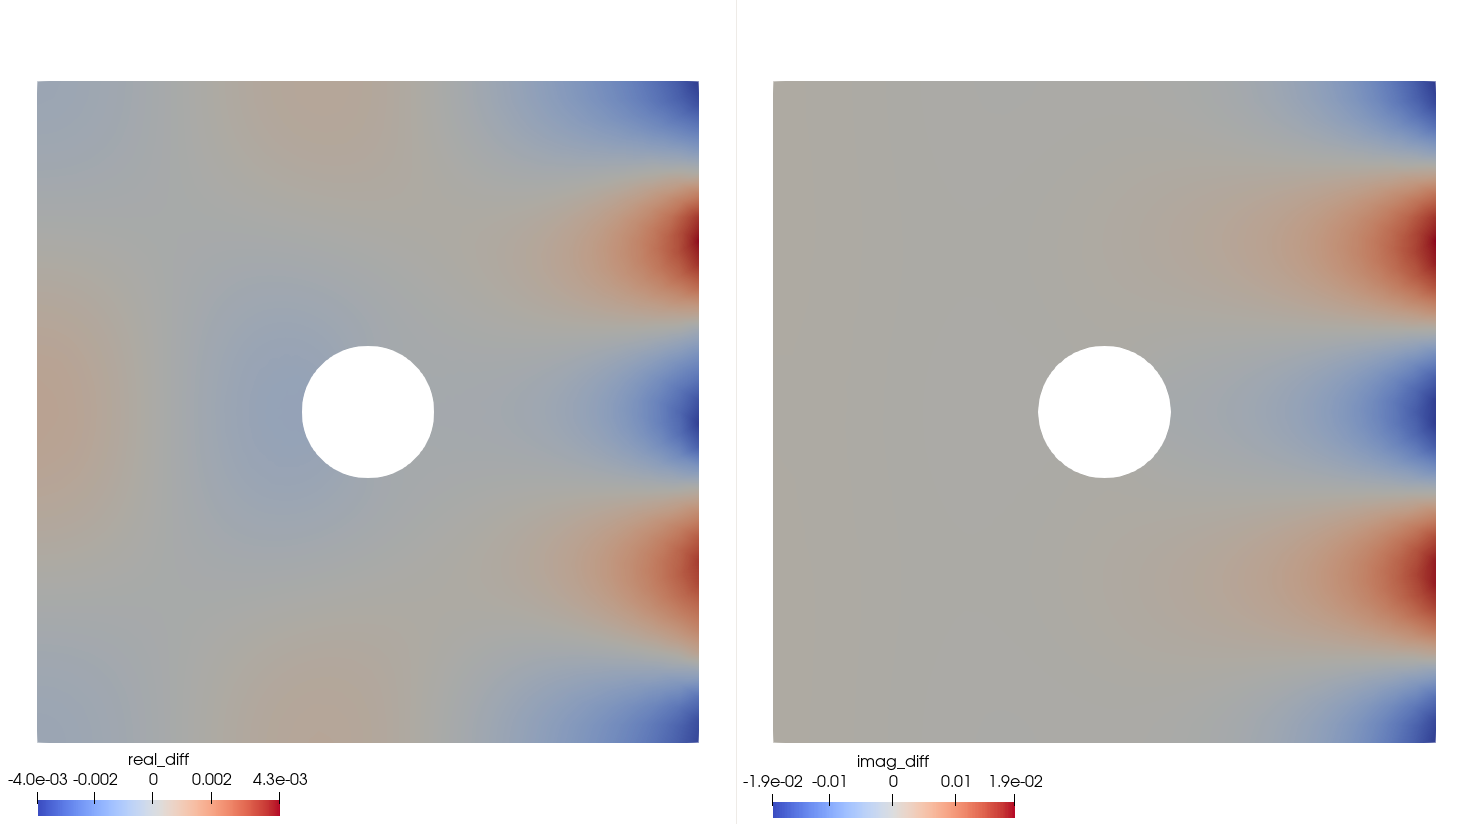
\includegraphics[scale=0.2]{sc_DtN_1_diff.png}
    \caption{$\mathfrak{Re }\; (u_{4}-u_{16})$ (haut), $\mathfrak{Im }\; (u_{4}-u_{16})$ (bas), $k=10$, $h=1$,  $a=1$}
\end{figure}


\subsection{Méthode DtN épais}
\subsubsection{Formulation variationnelle}

On introduit l'opérateur DtN épais tronqué $$
\tilde{T}_N u=\sum_{n=0}^N i \beta_n e^{i \beta_n(b-a)}\left(\int_{\Sigma_a} u \varphi_n\right) \varphi_n(y) \text { sur } \Sigma_b \quad (b>a)
$$
La formulation variationnelle devient :
Trouver $p \in H^1\left(\Omega_b\right)$, tel que $\forall q \in H^1\left(\Omega_b\right)$,
$$
\int_{\Omega_b}\left(\nabla p \cdot \nabla \bar{q}-k^2 p \bar{q}\right)-\int_{\Sigma_b}\tilde{T}_N p\bar{q}=\int_{\Sigma_{0}} g \bar{q} .
$$ 

\subsubsection{Résultats numériques}

\subsection{Méthode PML}
\subsubsection{Formulation variationnelle}


En introduisant la fonction
$$
\tilde{\alpha}(x)= \begin{cases}1 & \text { si } x<a \\ \alpha & \text { si } a<x<b\end{cases}
$$
où 
$$
\mathfrak{Re } \; \alpha>0 \text { et } \mathfrak{Im } \;  \alpha<0 \text {. }
$$ on obtient  le problème PML dans $\displaystyle \Omega_b$:
$$
\displaystyle
\begin{cases}\displaystyle \frac{\partial^2 u}{\partial y^2}+\tilde{\alpha} \frac{\partial}{\partial x}\left(\tilde{\alpha} \frac{\partial u}{\partial x}\right)+k^2 u=0 & \text { sur } \Omega_b \\[0.4cm] \displaystyle\frac{\partial u}{\partial n}=0 & \text { sur } \Gamma \cup \partial \mathcal{O} \cup \Sigma_b \\[0.4cm] \displaystyle \frac{\partial u}{\partial n}=g & \text { sur } \Sigma_0 \\[0.4cm] \displaystyle \frac{\partial u}{\partial n}=0 & \text { sur } \Sigma_b .\end{cases}
$$


La formule variationnelle associée est alors : Trouver $p \in H^1\left(\Omega_b\right)$, tel que $\forall q \in H^1\left(\Omega_b\right)$ $$ \int_{\Omega_b} \frac{1}{\tilde{\alpha}} \frac{\partial p_L}{\partial x} \frac{\partial \bar{q}}{\partial x}+\frac{1}{\tilde{\alpha}} \frac{\partial p_L}{\partial y} \frac{\partial \bar{q}}{\partial y}+\tilde{\alpha} \frac{\partial p_L}{\partial z} \frac{\partial \bar{q}}{\partial z}-\frac{k^2}{\tilde{\alpha}} p \bar{q}=\int_{\Sigma_0} g \bar{q} d \gamma $$
\subsubsection{Résultats numériques}

\end{document}
